\documentclass{beamer}

\usepackage{beamerthemesplit}
\usepackage{verbatim}

%\definecolor{MyGreen}{RGB}{60, 140, 60}
\definecolor{DarkPurple}{RGB}{60, 30, 60}
\definecolor{Gray90}{RGB}{230, 230, 230}
\definecolor{Gray10}{RGB}{25, 25, 25}


\usetheme{Pittsburgh}
%\usecolortheme{seagull}
%\usecolortheme{spruce}
%\usecolortheme{seahorse}
%\usecolortheme{beaver}
\setbeamercolor{structure}{fg=DarkPurple!90!black}
%\setbeamercolor{structure}{fg=Gray10!10!DarkPurple}

\usefonttheme{serif}

%\DeclareGraphicsExtensions{.pdf,.png,.jpg}

\newcommand{\snT}{$(S/N)_{\textrm{size}}$}
%\newcommand{\snT}{$\left( \frac{S}{N}\right)_{\textrm{size}}$}
\newcommand{\snflux}{$(S/N)_{\textrm{flux}}$}
%\newcommand{\snflux}{$\left( \frac{S}{N}\right)_{\textrm{flux}}$}

\newcommand{\lensfit}{\texttt{LENSFIT}}
\newcommand{\numba}{\texttt{Numba}}
\newcommand{\python}{\texttt{Python}}
\newcommand{\ngmix}{\texttt{ngmix}}
\newcommand{\shear}{{\bf g}}


% http://texblog.net/latex-archive/plaintex/beamer-footline-frame-number/
% to add the page (frame ) number and not screw up the bottom line
% works for split themes?
\expandafter\def\expandafter\insertshorttitle\expandafter{%
      \insertshorttitle\hfill%
        \insertframenumber\,/\,\inserttotalframenumber}


\begin{document}

%\frame{\titlepage}

%\section{DES Shear Pipelines}

\title{DES Shear Pipelines}
\author{Erin Sheldon}
\institute{Brookhaven National Laboratory}
\date{DES Collaboration Meeting, Sussex, 2014-10-20}

\frame{\titlepage}

\frame
{
    \frametitle{Outline}

    \begin{itemize}

        \item Brief description of the data and pipelines.
        \item Systematics tests
            \begin{itemize}
                \item Simulation based
                \item Data based (SVA1)
            \end{itemize}
        \item Summary
    \end{itemize}
}
 
\frame
{
    \frametitle{Pipelines}

    % \fontsize{9}{0.8\baselineskip}
    \begin{itemize}
        \item Two pipelines:
            \begin{itemize}
                \item im3shape: maximum likelihood fitter (Zuntz et al.)
                \item ngmix: bayesian shear estimation (Sheldon)
            \end{itemize}

        \item Algorithms are run on all epochs simultaneously: PSF is
            better behaved and understood on the single-epoch images.

        \item We use Multi-Epoch Data Structures for our processing (MEDS).
            MEDS files include:
            \begin{itemize}
                \item all postage stamps from all epochs associated with
                    each coadd object.
                \item weight maps
                \item bit masks
                \item other metadata
            \end{itemize}

        \item We only use coadds for detection.

    \end{itemize}
}

\frame
{
    \frametitle{Noise Bias}

    \begin{itemize}

        \item Using point estimates for shear can result in ``noise bias'', a
            calibration error that depends on S/N.

        \item GREAT DES simulations were created to test noise bias (Kacprzak)

        \item {\bf {\em im3shape:}}  measure noise bias and correct for it.

        \item {\bf {\em ngmix:}} no detectable noise bias

    \end{itemize}

    \begin{center}
        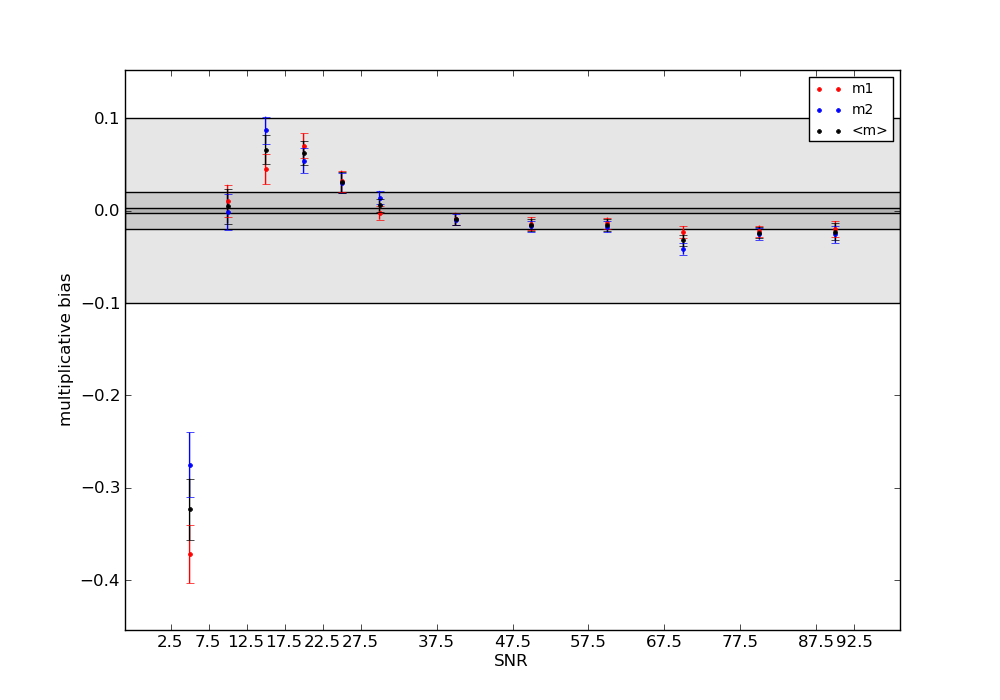
\includegraphics[width=0.5\textwidth]{noise-bias-im3shape.png}
        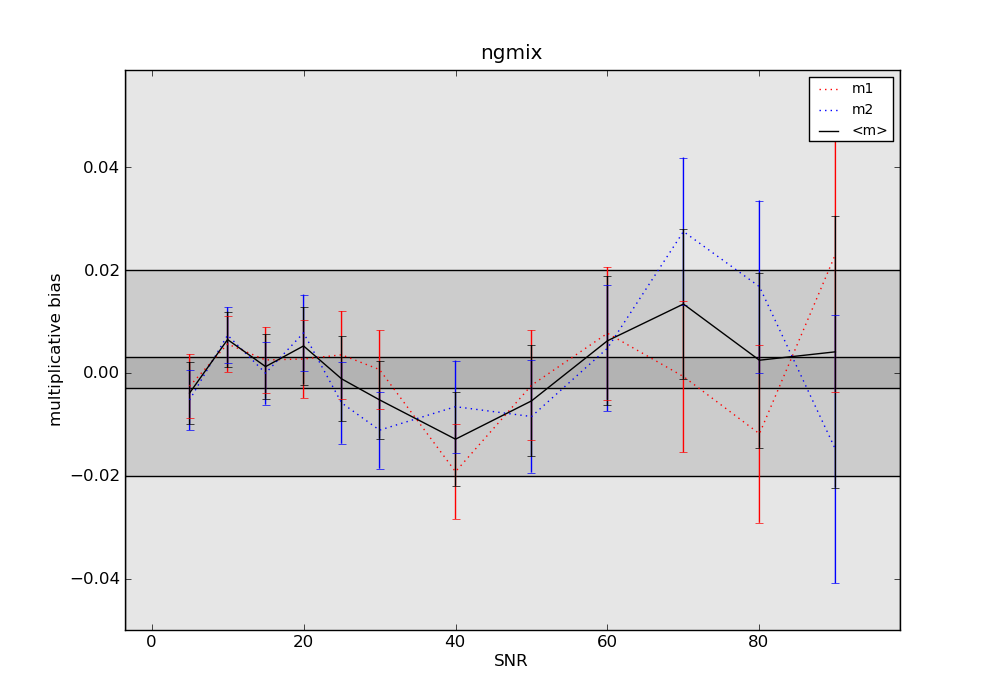
\includegraphics[width=0.5\textwidth]{noise-bias-ngmix.png}
    \end{center}
    {\tiny (Figures: Tomasz Kacprzak)}
}

\frame
{
    \frametitle{PSF Leakage}

    PSF Correction: Look for correlation between galaxy shape and PSF shape.

    \begin{columns}
        \begin{column}{0.38\textwidth}
            \begin{center}
                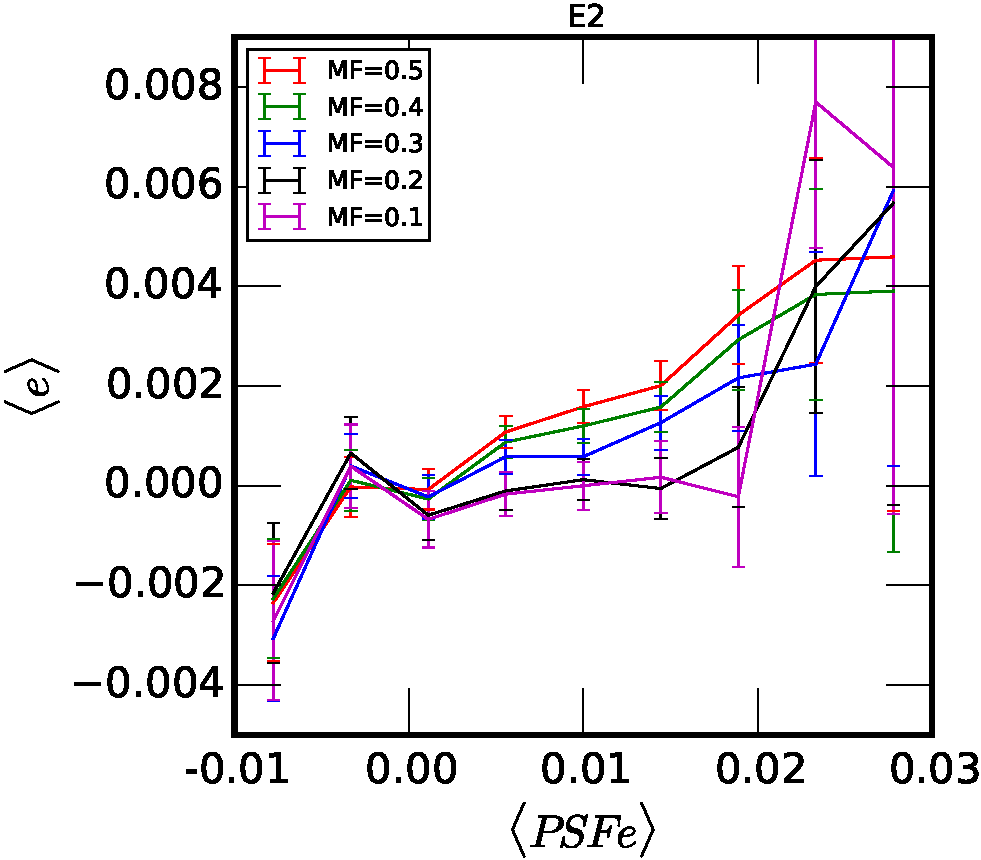
\includegraphics[width=\textwidth]{im3shape-PSF-E2.pdf}
                \newline
                {\tiny Figure: Vinu Vikram (im3shape)}
            \end{center}
        \end{column}
        \begin{column}{0.62\textwidth}
            \begin{center}
            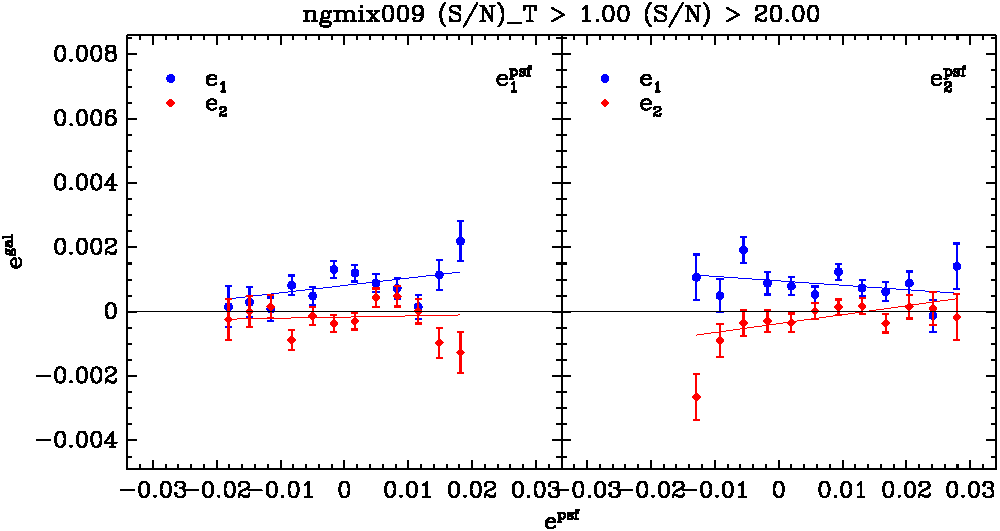
\includegraphics[width=\textwidth]{ngmix009-e-vs-epsf-Ts2n-min-1-s2n-min-20.pdf}
                \newline
                {\tiny Figure: Erin Sheldon}
            \end{center}
        \end{column}
    \end{columns}
}

\frame
{
    \frametitle{Random Points}

    Look for spurious signal round random points

    \begin{center}
        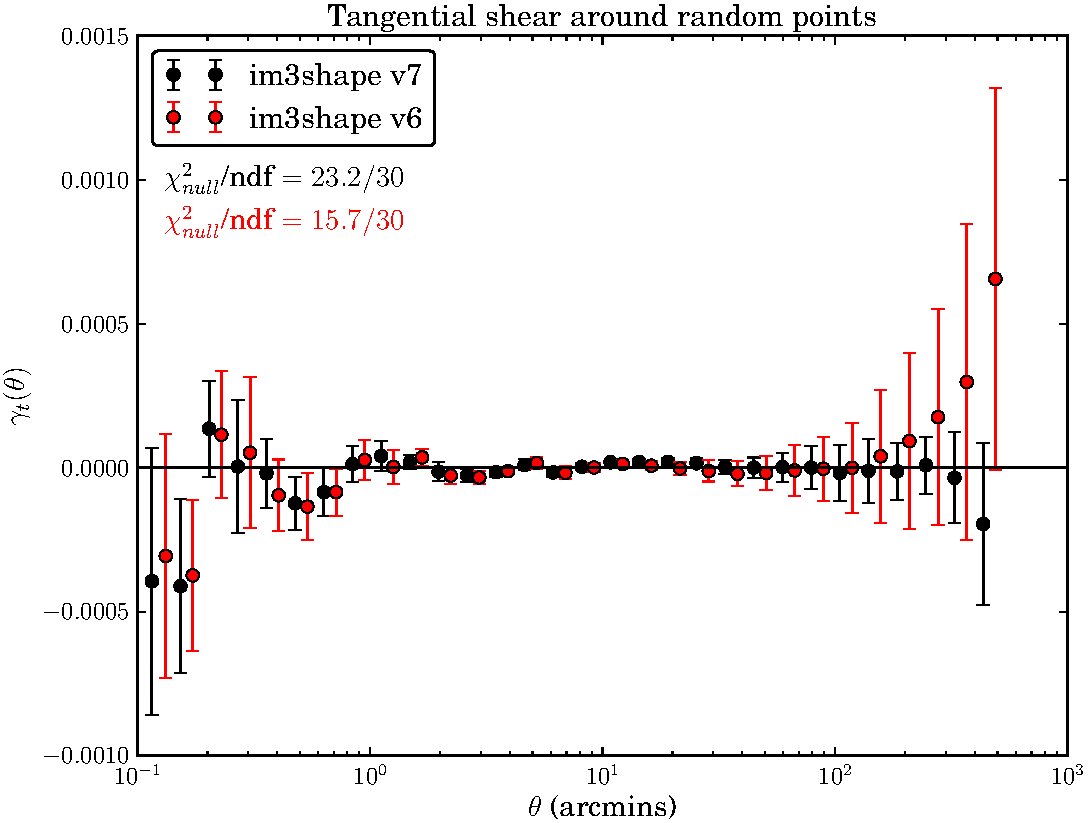
\includegraphics[width=0.7\textwidth]{random_points_v6_v7_crop.pdf}
    \end{center}
    {\tiny Figure: Carles S\`{a}nchez}
}

\frame
{
    \frametitle{B Modes}

    Gravity only produces an E mode shear polarization (shears transform like
    polarizations).  B mode should be consistent with zero.  These data are
    {\bf blinded}

    \begin{columns}
        \begin{column}{0.5\textwidth}
            \begin{center}
                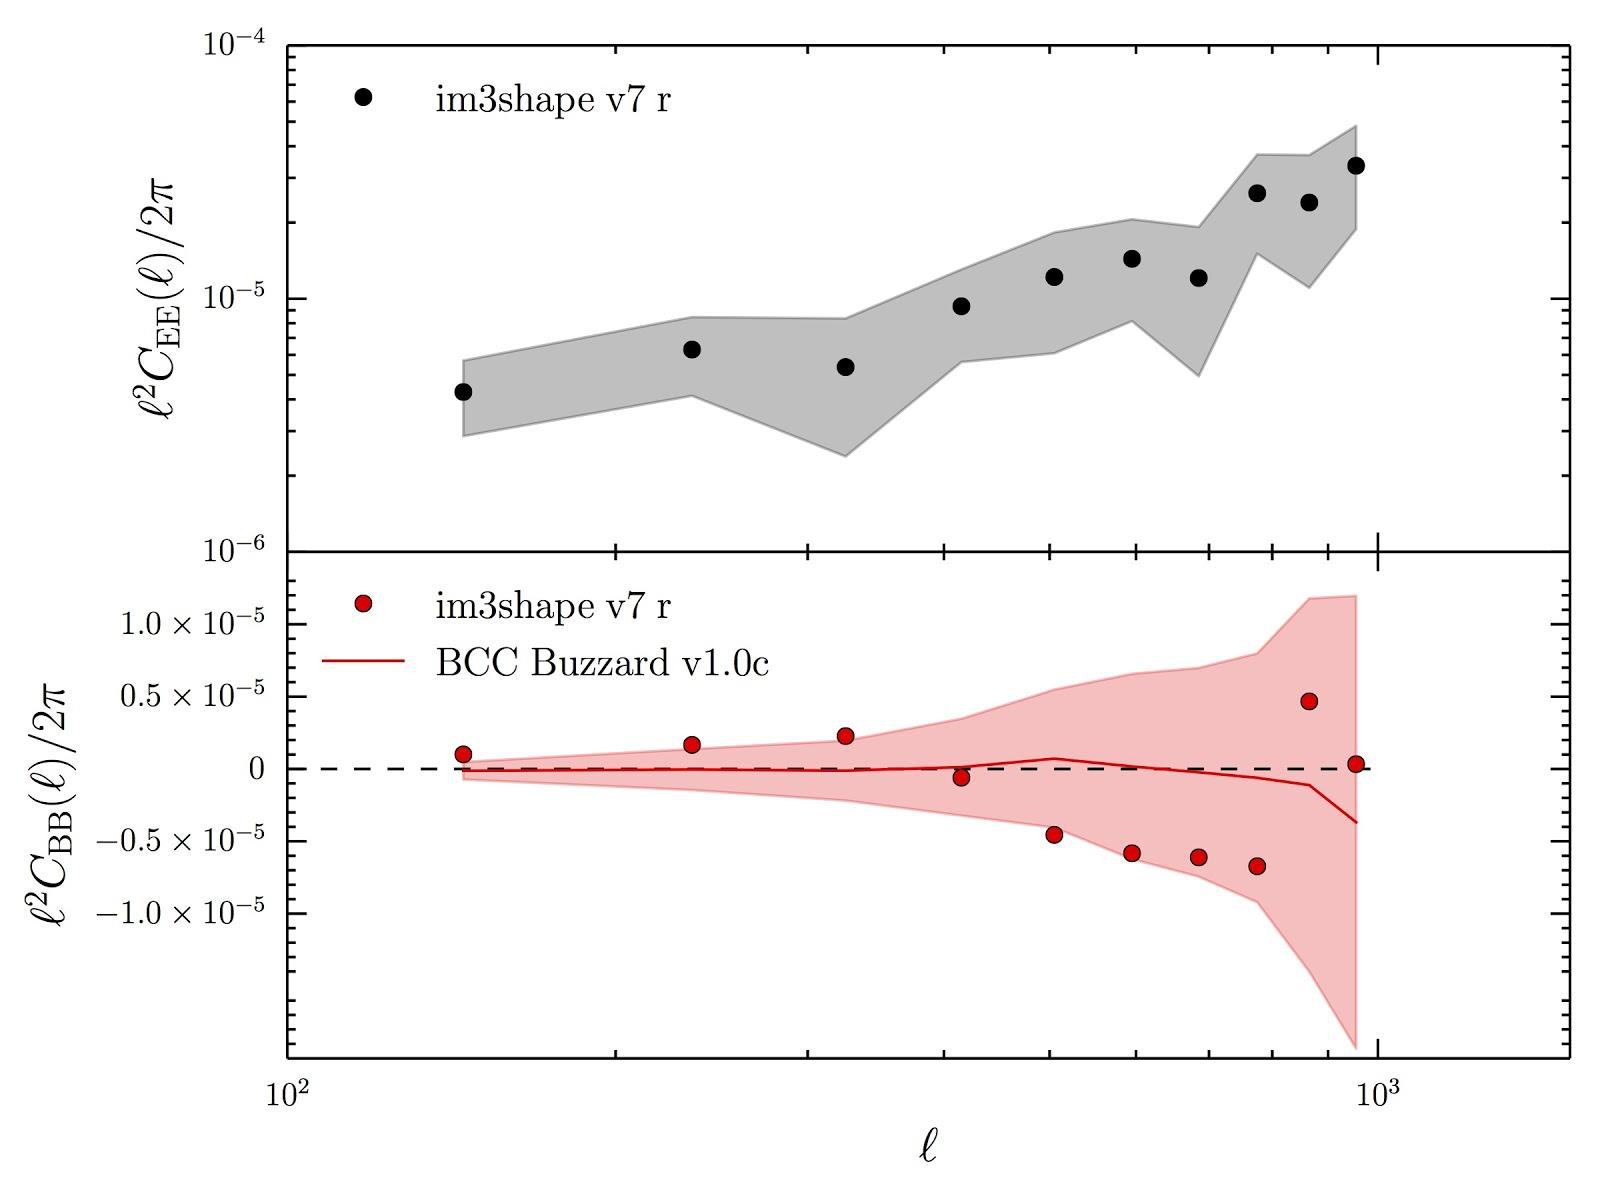
\includegraphics[width=\textwidth]{bmode-im3shape.png}
            \end{center}
        \end{column}
        \begin{column}{0.5\textwidth}
            \begin{center}
                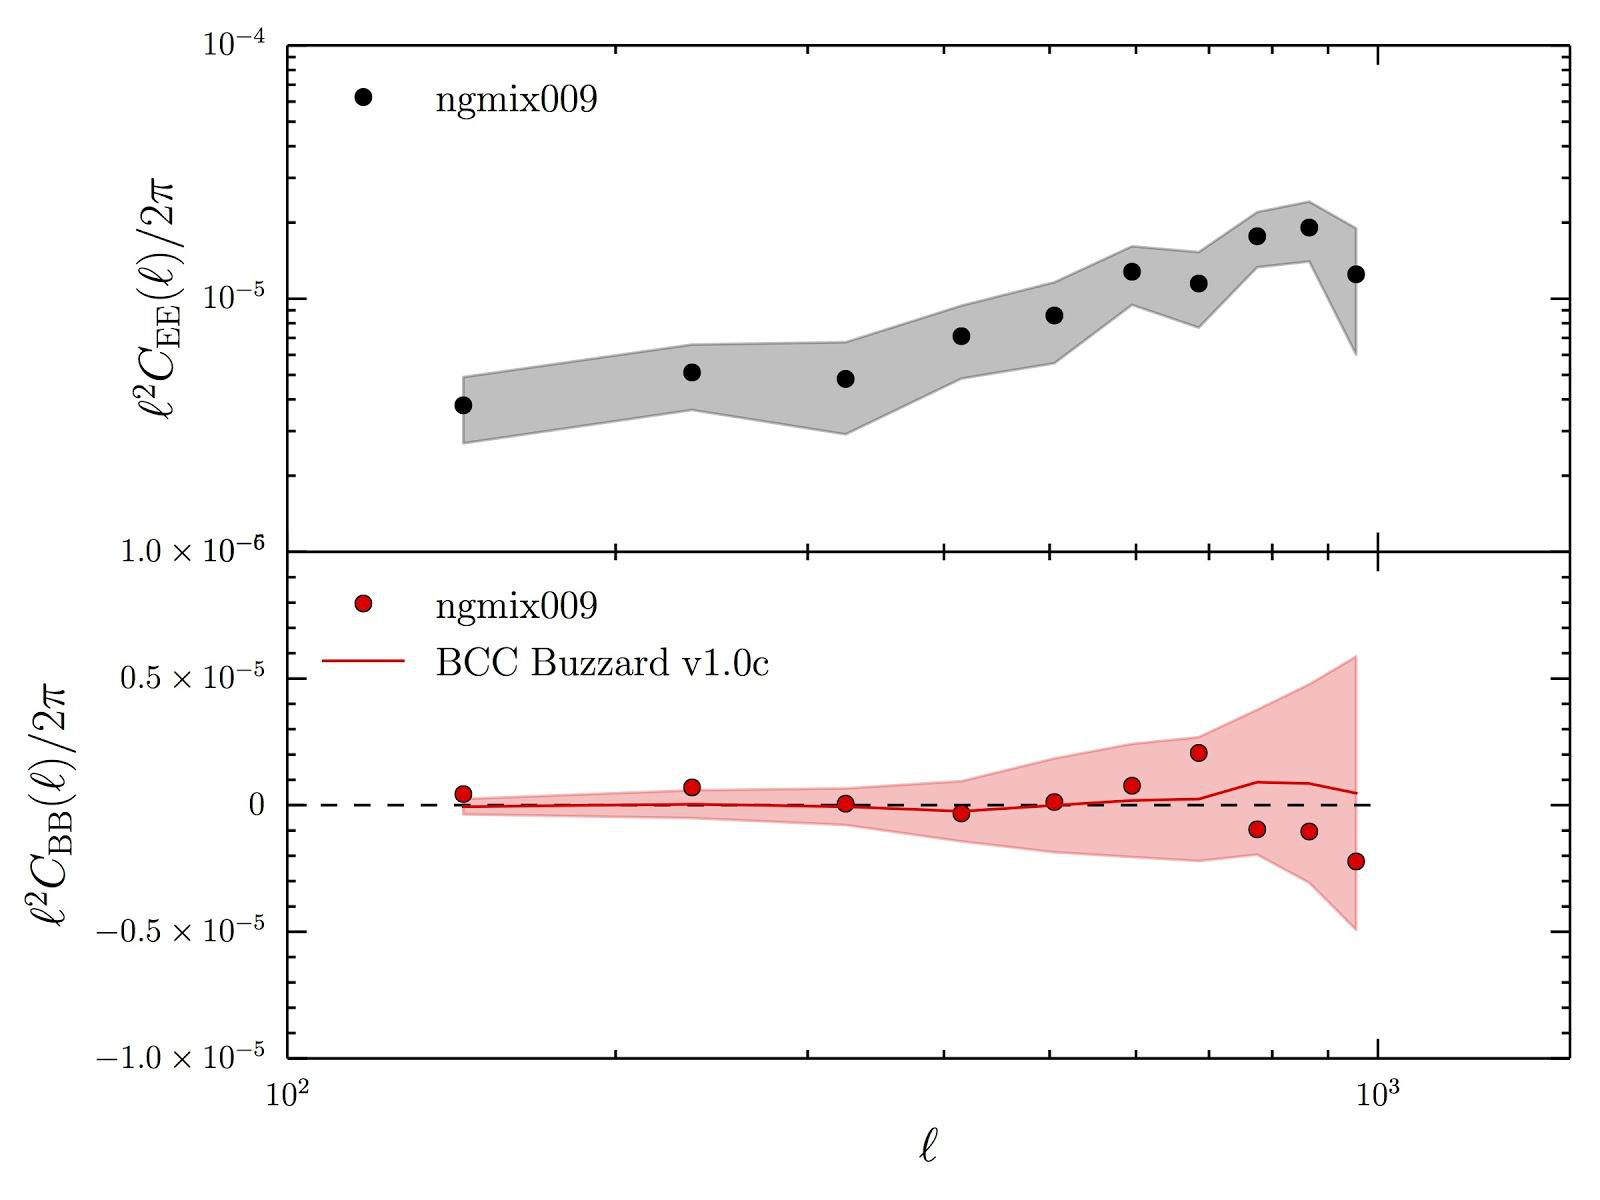
\includegraphics[width=\textwidth]{bmode-ngmix.png}
            \end{center}
        \end{column}
    \end{columns}
    {\tiny Figures: Matt Becker}
}

\frame
{
    \frametitle{Unexplained Systematics}

    \begin{itemize}

        \item Overall the null tests look good, but there are a few unexplained
            correlations.

        \item Measured galaxy shape correlates with the size of the postage stamp
    
         \item Measured galaxy shape correlates with the fraction of the stamp
             used for measurement, a.k.a the {\em masked fraction}.

     \end{itemize}

    \begin{center}
        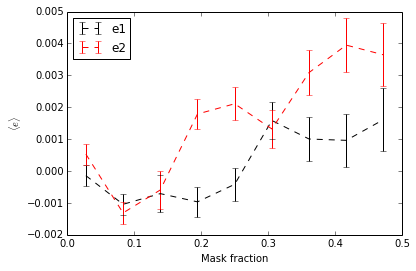
\includegraphics[width=0.5\textwidth]{im3shape-v-vs-mask-frac.png}
    \end{center}

     {\tiny Figure: Vinu Vikram (im3shape)}
}

\frame
{
    \frametitle{Summary}

    \begin{itemize}

        \item Overall the shear null tests look good.

        \item We do not currently see any show stoppers for lensing with SVA1 data.

    \end{itemize}
}


\end{document}
